\documentclass[12pt]{article}
\usepackage{graphicx}
\usepackage{fancyhdr}
\usepackage{amssymb}
\usepackage{amsmath}
\usepackage{array}
\usepackage{float}
\usepackage{caption}
\usepackage{subcaption}
\usepackage{lscape}
\usepackage[margin=1in]{geometry}
\usepackage{booktabs}
\usepackage{tikz}
\usetikzlibrary{positioning}
\usepackage{amsfonts}
\usepackage{amsthm}
\usepackage[utf8]{inputenc}
%\usepackage[backend=biber,style=numeric,sorting=none]{biblatex}
\usepackage[normalem]{ulem}
\usepackage{gensymb}
\usepackage{siunitx}
\usepackage{chemfig}
\usepackage{lastpage}
\usepackage{verbatim}
\usepackage{multirow}
\usepackage{graphicx}
\usepackage{microtype}
\usepackage{mathtools}
%\usepackage{float}
%\usepackage{subfigure}
%\usepackage[caption = false]{subfig}
\usepackage{amstext} % for \text macro
\newcolumntype{L}{>{$}l<{$}} % math-mode version of "l" column type

\pagestyle{fancy}
\rhead{Page \thepage \ of \pageref{LastPage}}
\lhead{Team Skuas}


\title{Using Linear Cancer Networks to Model Hormone Therapy for Breast Cancer}
\author{Zane Billings\\Martin Chan\\Will Stiles}
\date{May 3, 2019}

\begin{document}

\maketitle

\begin{abstract}
    \noindent Breast cancer is an invasive disease caused by mutations in the cells of the breast which ultimately prevent apoptosis from occurring (essentially, controlled cell death). This causes the cells to grow rapidly into tumors which typically kill the host when left without treatment.  This paper will observe the application of hormone treatment therapy with the hope of reduction or elimination of cancerous tumors prior to or following surgery.
\end{abstract}

\tableofcontents
\pagebreak

\section{Introduction}
% Introduce the idea behind the Breast Cancer Therapy source document and break down what we will be discussing.
\indent\indent Breast cancer is the most common form of cancer found in women. Starting in the epithelial cells of the breast, the cancer spreads to the surrounding tissue. There are four types of breast cancer mentioned in the paper by McDuffie: endocrine receptor positive for estrogen (ER+), endocrine receptor positive for progesterone (PR+), HER2 positive (HER2+), or negative for each of the three.  Estrogen, progesterone, and HER2 are hormone molecules which stimulate the proliferation of breast epithelial tissue. Treatment typically involves the use of either radiation therapy, hormone therapy, targeted therapy, chemotherapy, surgery, or in many cases a combination of these treatments.  We will be primarily focusing on the application of hormone therapy.

Hormone therapy only works for hormone receptor positive forms of breast cancer and is typically used after surgery to prevent the recurrence of cancer.  Tamoxifen is a common drug used to prevent this recurrence, slow the spread of the cancer, and even prevent cancer in women at high risk of getting breast cancer.  Tamoxifen, a selective estrogen-receptor modulator (SERM), attaches itself to the ER+ cancer cells to prevent them from binding to estrogen. Without estrogen, cell division is hindered in the tumor cells, and ultimately, apoptosis (cell death) is triggered.

Modern cancer models rely on systems of first order differential equations to model the populations of healthy cells and cancer cells.  Werner proposed a new framework in which cancer develops from mutations in the developmental control networks~\cite{werner}.  With this he introduced the concept of cancer networks in which cancerous stem cells divide to produce tumor cells from instructions within their network.  These networks are considered linear in which a cancerous cell can either divide into itself or a tumor cell. We can then model the introduction of hormone treatment therapy into this kind of linear cancer system and analyze the changes in stability and strength of the model in response to the hormones.

\section{A Breast Cancer Model}
% Introduce the initial model as discussed in the source document
\indent\indent We will need to define a few populations in our system before we observe hormone interactions within the system.  Those that need to be accounted for include cancer stem cells $(x)$, tumor cells $(y)$, and healthy cells $(z)$ in the breast.  Therefore we can model a system designed roughly like the one listed below.

\begin{eqnarray*}
    \Dot{x} & = & \mbox{Cancerous stem cells,}\\
    \Dot{y} & = & \mbox{Cancerous tumor cells, and}\\
    \Dot{z} & = & \mbox{Healthy cells}
\end{eqnarray*}

We will then need to observe how each population changes within their ecosystem. Using a linear cancer model as discussed in the introduction, the cancerous stem cells will produce cancerous tumor cells at a linear rate.  Modeling the growth of all cells logistically, we get a system where the populations $x, y,$ and $z$ are limited by their population capacities $x_c, y_c, $ and $z_c$ respectively, where cancerous cells grow at a rate of $k$ and healthy cells at a rate of $q$.
\pagebreak 
Note that there will exist a natural death rate $n$ of tumor cells, since Werner indicates in his research that tumor cells are terminal and do not divide on their own. The resultant system can then be modelled by the following equations:

\begin{eqnarray*}
    \Dot{x} & = & kx\Big( 1-\frac{x}{x_c}\Big)\\
    \Dot{y} & = & kx\Big( \frac{x}{x_c}\Big)\Big( 1-\frac{y}{y_c}\Big) - ny\\
    \Dot{z} & = & qz\Big( 1-\frac{z}{z_c}\Big)
\end{eqnarray*}

This will model the cancerous system without any sort of treatment.  We will begin by performing an analysis of the equilibria on the current system. We can then consider adding hormone therapy to the model and observe what transpires.

%\subsection{Parameterization of the Model}
% Discuss the parameters of the model and determine which parameters will be adjusted (likely the Tamoxifen dosage and effectiveness


\subsection{Equilibria, the Jacobian Matrix, and Eigenvalues}
\indent\indent Without introducing estrogen-dependent growth and hormone therapy into the model, the cancer system behaves similarly to a three-population logistic Lotka-Volterra model.  There are four equilibria for the model. By taking 
\begin{eqnarray*}
    0 & = & kx\Big( 1-\frac{x}{x_c}\Big)\\
    0 & = & kx\Big( \frac{x}{x_c}\Big)\Big( 1-\frac{y}{y_c}\Big) - ny\\
    0 & = & qz\Big( 1-\frac{z}{z_c}\Big),
\end{eqnarray*}
\noindent
we obtain four solutions:
\begin{equation}
    \left( 0, 0, 0 \right),
\end{equation}
\begin{equation}
    \left( 0, 0, z_c \right),
\end{equation}
\begin{equation}
    \left( x_c, \frac{kx_cy_c}{kx_c+y_cn}, 0 \right),
\end{equation}
and
\begin{equation}
    \left( x_c, \frac{kx_cy_c}{kx_c+y_cn}, z_c \right). 
\end{equation}

\noindent The Jacobian matrix for the model was calculated as
\[J=
\begin{bmatrix}
k\left(1-\frac{x}{x_c}-\frac{kx}{x_c}\right) & 0 & 0 \\
2k\frac{x}{x_c}\left(1-\frac{y}{y_c}\right) & -\frac{kx^2}{x_cy_c}-n & 0 \\
0 & 0 & q\left(1-\frac{z}{z_c}\right)-q\frac{z}{z_c}
\end{bmatrix}.
\]

By evaluating the Jacobian matrix at each of the equilibrium values and then computing the eigenvalues of the resulting matrix, we determine the stability of each of the equilibrium points.

\begin{table}[h!]
\centering
\caption{The eigenvalues of the Jacobian evaluated at each of the four equilibria.}
\begin{tabular}{|c|c|c|c|}
\hline
Equilibrium & \(\lambda_1\) & \(\lambda_2\) & \(\lambda_3\)\\
\hline
\hline
1 & $k$ & $-n$ & $q$ \\
\hline
2 & $k$ & $-n$ & $-q$ \\
\hline
3 & $-k$ & $-\frac{kx_c+ny_c}{y_c}$ & $q$ \\
\hline
4 & $-k$ & $-\frac{kx_c+ny_c}{y_c}$ & $-q$ \\
\hline
\end{tabular}
\label{t:notreatmenteigs}
\end{table}

\subsection{Stability of Equilibria}
\indent\indent Interestingly, the origin displays saddle behavior rather than the source behavior typical of most dynamic population models (e.g. three population Lotka-Volterra). The eigensystem at the origin suggests that while there is source behavior for both the cancer stem cells and the healthy epithelial cells, the cancer tumor cells have slightly more complicated behavior about the origin; it appears that in the linearized system, the cancer tumor cell will always decline. However, the linearized version does not take into account the dependency of the tumor cell population on the cancer stem cell population.

In the unstable second equilibirium point, there are no cancer cells. The population of healthy cells rises to their natural carrying capacity, but if any cancer cells are introduced into the system, the solution trajectories of the system will be repelled by this equilibrium (that is, it will be a saddle point).

Finally, the fourth equilibrium point represents an asymptotically stable equilibrium of coexistence. The basin of attraction for the equilibrium point is difficult to determine, but visually, it appears to be in the first octant. 
% \begin{figure}[h!]
%     \centering
%     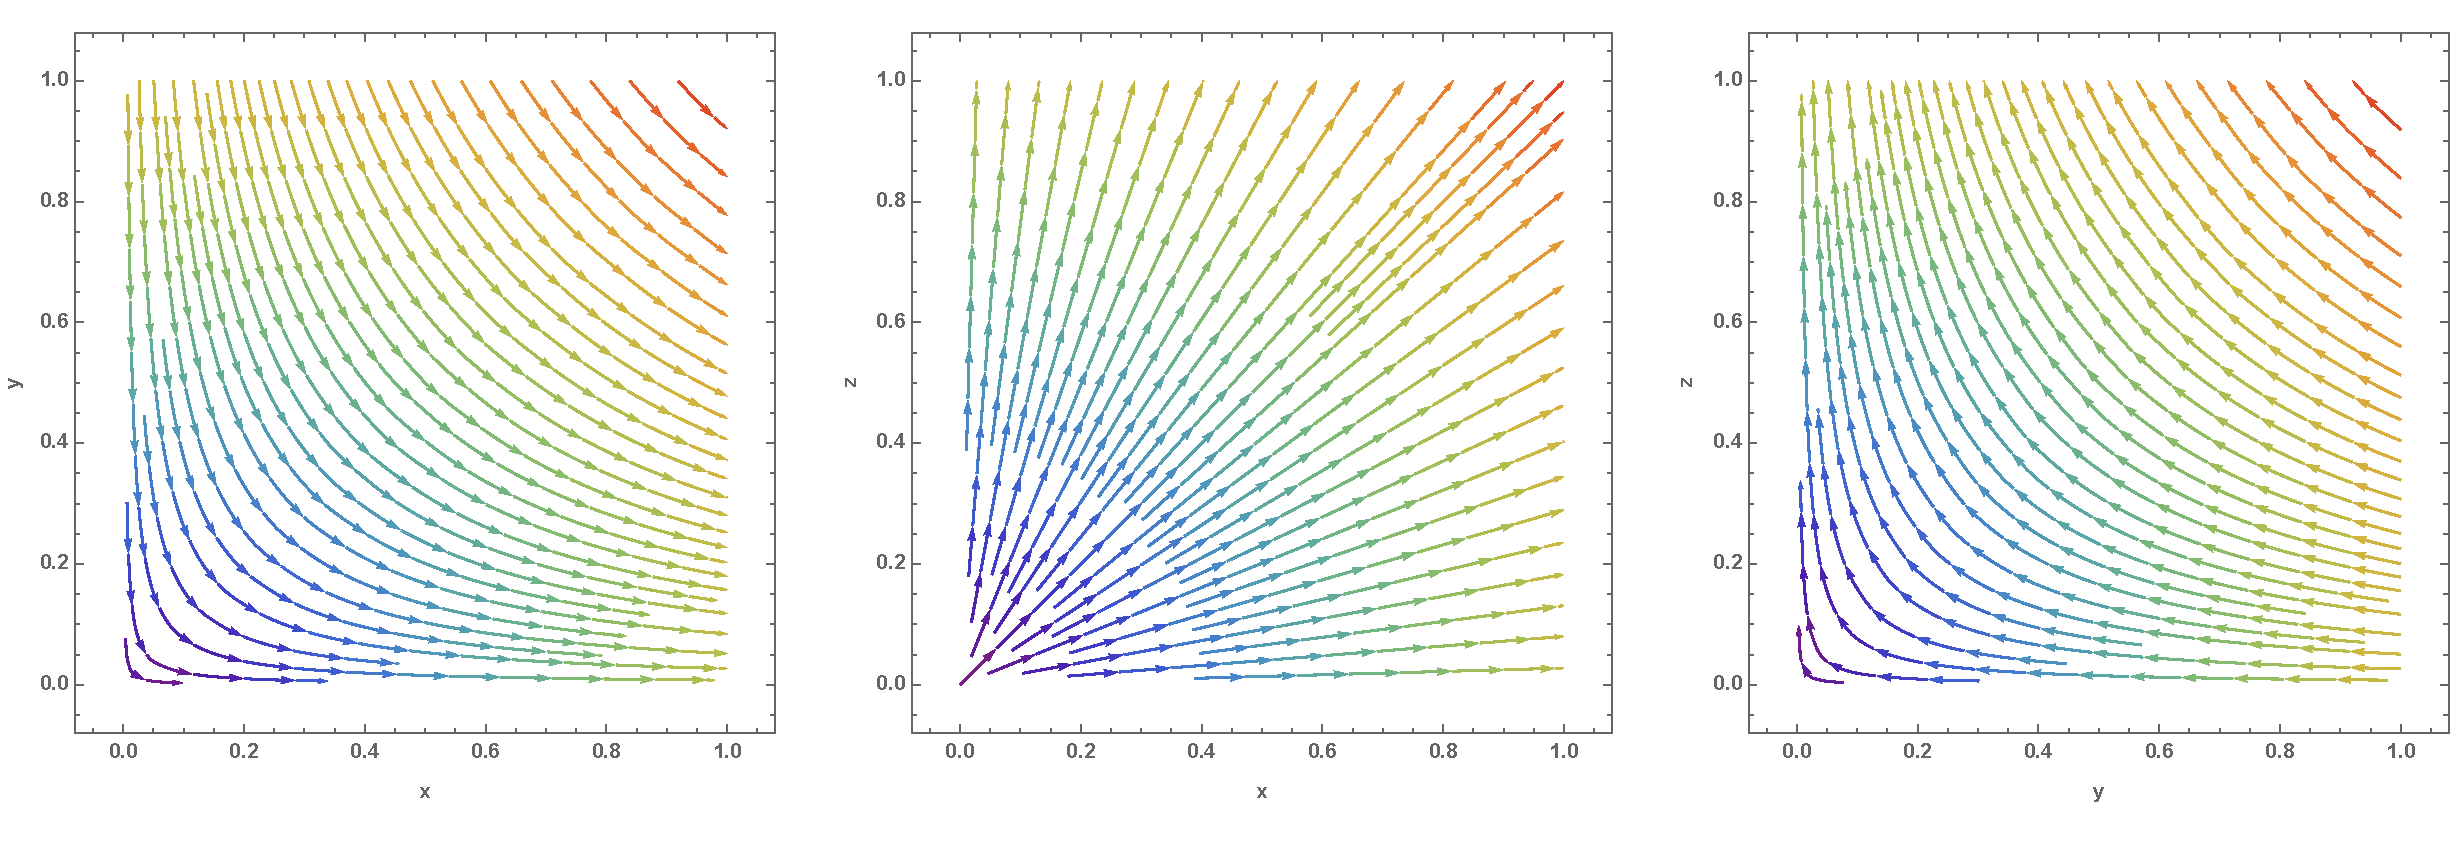
\includegraphics[width=0.9\textwidth]{NoTreatmentSlicesOrigin.pdf}
%     \caption{Projections onto each of the center planes of the linearized system about the origin. }
%     \label{fig:notreatmentorigin}
% \end{figure}

\subsection{Introduction of Estrogen Level}
\indent\indent When we introduce estrogen to the system as well as Tamoxifen hormone therapy, adding an estrogen level component $(w)$ to the system and observing the changes from the initial model.  With the introduction of this hormone we are left with the following system:

\begin{eqnarray*}
    \Dot{x} & = & \Big( \frac{kw}{w_0}\Big) x\Big( 1-\frac{x}{x_c}\Big) - d_1\Big( 1- \frac{w}{w_0}\Big)x\\
    \Dot{y} & = & \Big( \frac{kw}{w_0}\Big) x\Big( \frac{x}{x_c}\Big)\Big( 1-\frac{y}{y_c}\Big) - ny - d_2\Big( 1- \frac{w}{w_0}\Big)y\\
    \Dot{z} & = & \Big( \frac{qw}{w_0}\Big) z\Big( 1-\frac{z}{z_c}\Big) - d_3\Big( 1- \frac{w}{w_0}\Big)z\\
    \Dot{w} & = & rw\Big(1 - \frac{w}{w_0}\Big) - sDw .
\end{eqnarray*}

Notice that the estrogen level directly affects the growth and death rate of each type of cell.  With $w$ representing the amount of estrogen that is available to bind to receptors, and $w_0$ representing the amount of estrogen necessary for the cells to divide normally.  Naturally since we have an expected level of estrogen, then the growth and death rates of the cells will fluctuate based on the level of estrogen compared to the expected level.  This will introduce an adjusted death rate for each cell population based on the comparable level of estrogen to the expected level, the rates being represented by $d_1, d_2,$ and $d_3$.

We then introduce a fourth equation for the change in estrogen level with respect to time. This will also be represented by a logistic growth model, where $r$ will represent the growth rate of the receptor binding estrogen.  Along with the introduction of Tamoxifen, we will adjust by a dosage $(D)$ of the drug as well as the effectiveness of the drug $s$ given the estrogen level. 

Now it is likely very apparent to the reader that both the size of the system and number of parameters are quickly getting out of hand.  So the next step will be to reduce the number of components in the model to make analysis much more manageable.

\section{A Dimensionless Model}
% Construct the dimensionless model here and explain the new system.
\indent\indent We can reduce the number of terms by converting the initial model listed by McDuffie~\cite{mcduffie} to a dimensionless system with populations listed as proportions of the carrying capacity, as well as the consolidation of certain similar parameters. In doing so we are able to reduce to the following system.

\begin{eqnarray*}
    \Dot{x} & = & wx(1 - x) - \delta_1(1 - w)x\\
    \Dot{y} & = & \mu wx^2(1 - y) - \eta y - \delta_2(1 - w)y\\
    \Dot{z} & = & \gamma wz(1 - z) - \delta_3(1 - w)z\\
    \Dot{w} & = & \rho (1 - w)w - \sigma w ,
\end{eqnarray*}

\noindent where

\begin{align*}
    x &= \frac{x}{x_c}, &\delta_i =& \frac{d_i}{k}, i = 1,2,3,\\
    y &= \frac{y}{y_c}, &\eta =& \frac{n}{k},\\
    z &= \frac{z}{z_c}, &\gamma =& \frac{q}{k},\\
    w &= \frac{w}{w_c}, &\rho =& \frac{r}{k},\\
    \mu &= \frac{x_c}{y_c}, &\sigma =& \frac{sD}{k}.
\end{align*}

For analysis purposes, the values used for the parameters will be listed in Table 2, given by McDuffie (p. 154).

\begin{table}
\centering
\caption{Fixed parameters for numerical and stability analysis}
\begin{tabular}{|c|c|}
\hline
Parameter & Values \\
\hline
\hline
$\rho$ & 0.40 \\
\hline
$\gamma$ & 0.75 \\
\hline
$\delta_1$ & 0.55 \\
\hline
$\delta_2$ & 0.65 \\
\hline
$\delta_3$ & 0.20 \\
\hline 
$\mu$ & 0.50 \\
\hline 
$\eta$ & 0.25 \\
\hline 
\end{tabular}
\end{table}

\vspace{.5in}

\subsection{Equilibria of the Dimensionless System}
% Determine equilibria of the new system and determine stability.
\indent\indent Similarly, with this new dimensionless system, we can determine the equilibria, the Jacobian matrix, and its eigenvalues. There are five equilibria for this model. By taking  

\begin{align*}
    0 &= w x (1-x) - \delta_1 (1-w) x \\
    0 &= \mu w x^2 (1-y) - \eta y - \delta_2 (1-w) y \\
    0 &= \gamma w z (1-z) - \delta_3 (1-w) z \\
    0 &= \rho (1-w) w - \sigma w,
\end{align*}

\noindent we can obtain five solutions:

\begin{equation}
    \left(0,0,0,0\right),
\end{equation}
\begin{equation}
    \left(0,0,0, \frac{\rho - \sigma}{\rho}\right),
\end{equation}
\begin{equation}
    \left(\frac{\rho - \sigma - \delta_1 \sigma}{\rho - \sigma}, \frac{\mu (\rho - \sigma - \delta_1 \sigma)^2}{\mu (\rho - \sigma - \delta_1 \sigma)^2 + (\rho - \sigma)(\eta \rho + \delta_2 \sigma)}, 0, \frac{\rho - \sigma}{\rho} \right), 
\end{equation}
\begin{equation}
    \left(0,0, \frac{\gamma \rho - \gamma \sigma - \delta_3 \sigma}{\gamma (\rho - \sigma)}, \frac{\rho - \sigma}{\rho} \right),
\end{equation}
\begin{equation}
    \left (\frac{\rho - \sigma - \delta_1 \sigma}{\rho - \sigma}, \frac{ \mu (\rho - \sigma - \delta_1 \sigma)^2}{\mu (\rho - \sigma - \delta_1 \sigma)^2 + (\rho - \sigma)(\eta \rho + \delta_2 \sigma)}, \frac{\gamma \rho - \gamma \sigma - \delta_3 \sigma}{\gamma (\rho - \sigma)}, \frac{\rho - \sigma}{\rho} \right).
\end{equation}\\

\noindent The Jacobian matrix was found to be the following:\\

\[
J=
\begin{bmatrix}
    w - 2xw - \delta_1 + \delta_1 w & 0 & 0 & x-x^2+\delta_1 x \\
    2\mu w x - 2\mu w x y & -\mu w x^2 - \eta - \delta_2 + \delta_2 w & 0 & \mu x^2 - \mu x^2 y + \delta_2 y \\
    0 & 0 & \gamma w - 2\gamma w z - \delta_3 + \delta_3 w & \gamma z - \gamma z^2 + \delta_3 z \\
    0 & 0 & 0 & \rho - 2 \rho w - \sigma
\end{bmatrix}
\]

When evaluated at the cure state equilibrium, where the healthy cells and the level of estrogen coexists, with values of $(0,0,\bar{z}, \bar{w})$, where $\bar{z}=\frac{\gamma \rho - \gamma \sigma - \delta_3 \sigma}{\gamma (\rho - \sigma)}= \frac{1.\bar{3}(0.3-0.95\sigma)}{0.4-\sigma}$ and $\bar{w} = \frac{\rho - \sigma}{\rho} = 2.5(0.4-\sigma)$, the Jacobian matrix transforms into the following:

\[
\begin{bmatrix}
    1-3.875\sigma & 0 & 0 & 0 \\
    0 & -0.25-1.625\sigma & 0 & 0 \\
    0 & 0 & -0.75+2.375\sigma & \frac{0.032-0.1013\sigma}{(-0.4+\sigma)^2} \\
    0 & 0 & 0 & -0.4+\sigma
\end{bmatrix}.
\]

Its respective eigenvalues are found to be:

\begin{align*}
    \lambda_1 &= -0.4 + \sigma \\
    \lambda_2 &= -0.75 + 2.375\sigma \\
    \lambda_3 &= 1-3.875\sigma \\
    \lambda_4 &= -0.25 - 1.625\sigma . 
\end{align*}

For the equilibrium to be consider stable, all eigenvalues have to be negative. We will explore more on the parameter $\sigma$ in the next section. 

\subsection{Sensitivity of Parameters}
% Determine the sensitivity of the system to a change in amounts of sigma.
\indent\indent 
In order to investigate the effects of hormone therapy, we investigate the sensitivity of each of the equations in the dimensionless model to the dimensionless treatment parameter, \(\sigma\). This parameter takes into account the growth rate of cancer cells, the effectiveness of Tamoxifen, and the dosage of Tamoxifen used for treatment. 

Using the equilibria given by McDuffie~\cite{mcduffie}, the sensitivity of each value in the equilibrium to sigma was calculated. However, in symbolic form the calculations were not very useful, so the table of values given by McDuffie (p. 154) was used for numerical analysis of sensitivity (however, $\sigma$ was allowed to remain a variable so it could be analyzed further).

Using the given numerical parameter values, the sensitivity of the equilibrium point value is in terms of \(\sigma\) for all four of the equations. The equations are extremely large and difficult to understand analytically, so the value of the sensitivities were plotted for \(\sigma \in [0,\rho)\). (Recall, we assume that \(\sigma<\rho\) for all equilibria.)

\begin{figure}[p]
    \centering
    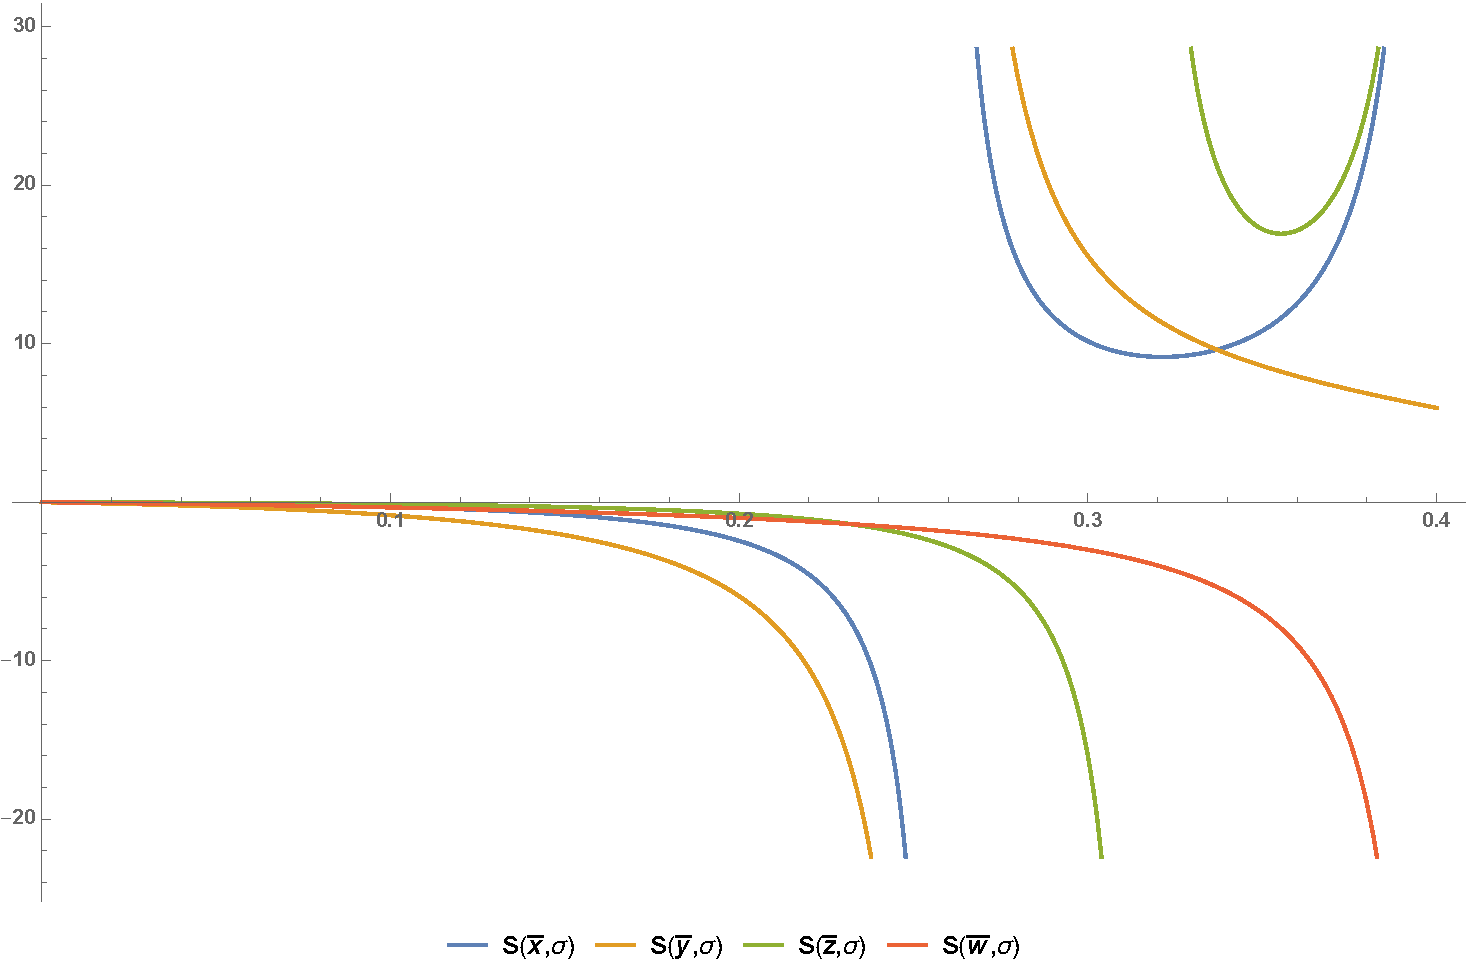
\includegraphics[width=0.9\textwidth]{SensitivitiesToSigma.pdf}
    \caption{Plot of the senstivity of each equilibrium point equation to \(\sigma\) as the value of \(\sigma\) increases.}
    \label{fig:sensitivitytosigma}
\end{figure}

By substituting McDuffie's parameter values into the equilibrium equations, we can qualitatively see how the sensitivities affect the change in the actual values of the population sizes over time.

\begin{figure}[p]
    \centering
    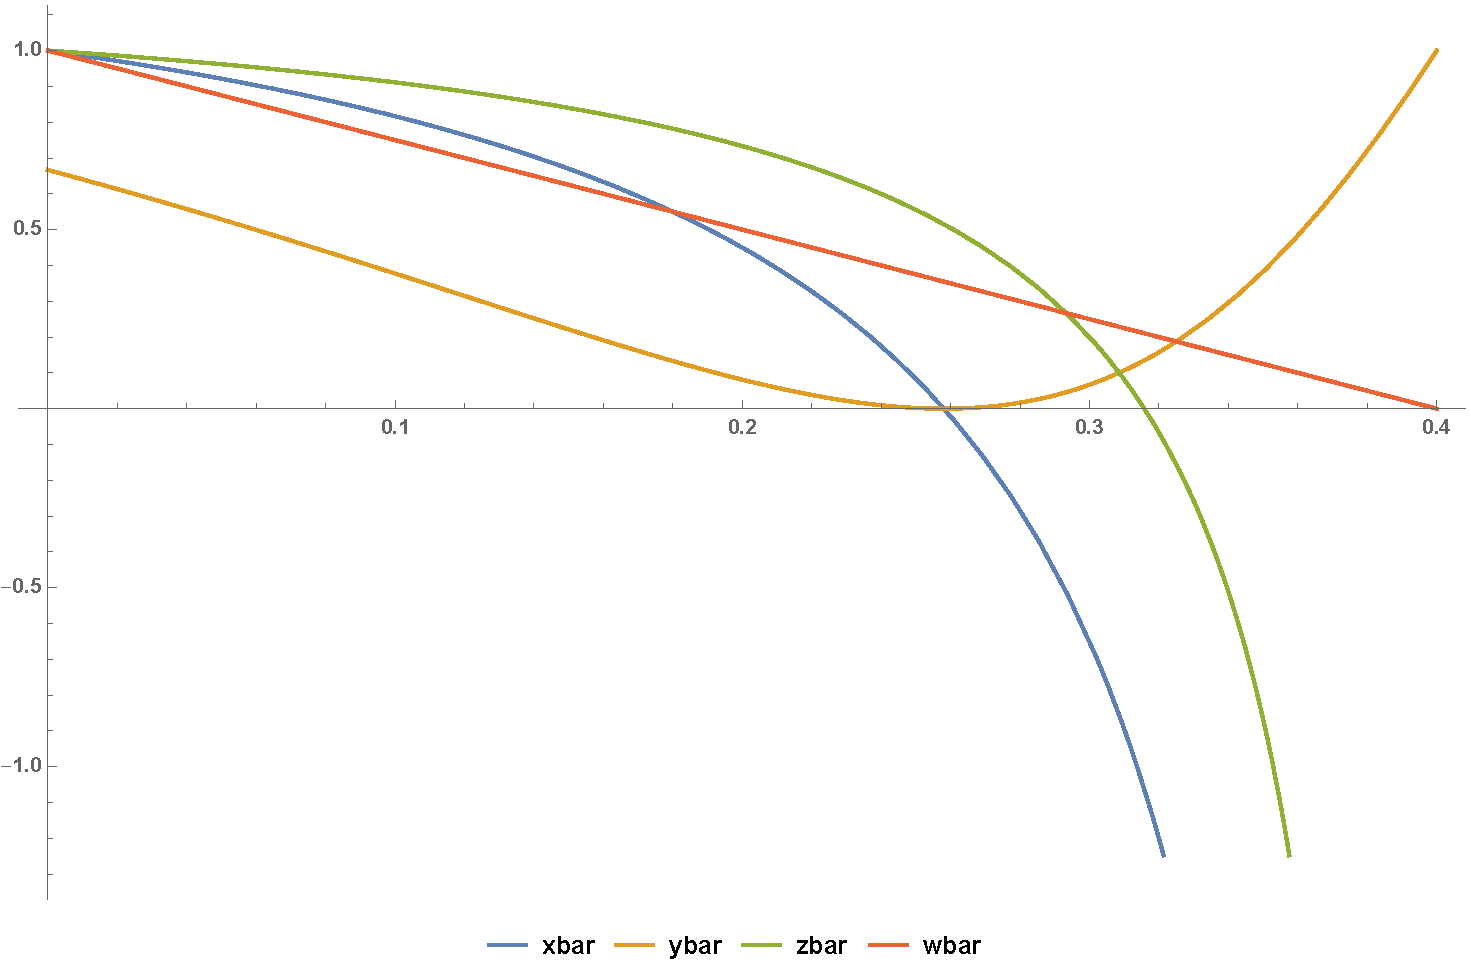
\includegraphics[width=0.9\textwidth]{ValuesVsSigma.pdf}
    \caption{The equilibrium values for each population change as \(\sigma\) varies over the interval [0,\(\rho\) = 0.4).}
    \label{fig:valuesvssigma}
\end{figure}

\subsection{Optimizing the Parameter \(\sigma\)}

\indent\indent Several conditions are given by McDuffie for the ``cure state'' (when there are only healthy cells and estrogen, no cancer cells) to be asymptotically stable. We have:
\begin{align*}
    \sigma &< \rho, \\
    \frac{\rho - \sigma}{\sigma} &< \delta_1, \\
    \frac{\gamma(\rho - \sigma)}{\sigma} &>\delta_3.
\end{align*}

Since \(\sigma\) encodes the dosage of Tamoxifen, an optimal value of \(\sigma\) should cause the cure state to be stable, and maximize the amount of remaining healthy cells. 

Rewriting the second constraints, we have that
\[\frac{\rho}{1+\delta_1} < \sigma < \frac{\rho}{1+\delta_3/\gamma}. \]

Substituting the parameter values given by McDuffie, we obtain
\[\frac{0.4}{1+0.55} < \sigma < \frac{0.4}{1+0.2/0.75},\]
approximately
\[0.258065 < \sigma < 0.315789.\]

To obtain a closed interval to be used for finding an optimal value of \(\sigma\), the approximation 
\[0.26 \leq \sigma \leq 0.31\]
was used.

Using this constraint, the objective function \(\bar{z}\), given earlier, can be optimized with respect to the parameter \(\sigma\). So, the parameters given were plugged into \(\bar{z}\), which was left in terms of \(\sigma\). 

By the Extreme Value Theorem, if a function is continuous over a closed interval, then it has an absolute maximum over that interval, and we also know that absolute extrema must occur at either an endpoint of the region or at a critical point of the function within the region.

In order to check \(\bar{z}(\sigma)\) for critical points over the region, we take
\[\bar{z}'(\sigma) = \frac{(4/3)(0.3-0.95\sigma)}{(0.4-\sigma)^2}-\frac{(19/15)}{0.4-\sigma}.\]

Note that \(\bar{z}(\sigma)\) is continuous (and differentiable) everywhere except for \(\sigma = 0.4\), which lies outside of the region and thus will not be problematic. There are no solutions for the equation \(\bar{z}=0\), and thus there are no critical points in the region (or elsewhere). Since there are no critical points of the function \(\bar{z}\) within the region, the absolute maximum must lie at one of the endpoints of the region.

Calculating the values at the two endpoints, we get 
\[\bar{z}(0.26) \approx 0.50 ;\ \bar{z}(0.31) \approx 0.08,\]
so the maximum over the region is the lower endpoint, \(\sigma = 0.26\). Numerically, we see that as the value of \(\sigma\) approaches the number \(0.4/1.55\), the value of \(\bar{z}\) continues to increase, indicating that the maximum value of \(\bar{z}\) lies at \(\sigma = 0.4/1.55\), but this will result in a zero eigenvalue, making the cure state no longer asymptotically stable.

So, the optimal value of \(\sigma\) is to be as close as possible to \(\sigma = 0.4/1.55\) without ever reaching this point. The approximation \(\sigma = 0.26\) ensures that the cure state is stable and approximates the maximal value of \(\bar{z}\) well.

Noting the previously calculated eigenvalues for the cure state, we can check to ensure that P4 remains stable.

\subsection{Using \(\sigma\) to Analyze Optimal Dosage}
\indent\indent The optimized parameter \(\sigma\) is dependent on three other parameters. Given the optimal value of \(\sigma\), the optimal dosage of tamoxifen can be viewed as a function of two variables. We have
\[\sigma = 0.26 = \frac{sD}{k} \implies D = \frac{0.26k}{s},\]
where \(D\) is the dosage of Tamoxifen, \(s\) is the effectiveness of Tamoxifen at blocking estrogen receptors, and \(k\) is the growth rate of cancer cells.

The sensitivity of optimal dosage to both parameters is easily obtained: the sensitivity of dosage to cancer growth rate is 1, and the sensitivity of dosage to Tamoxifen effectiveness is \(-1\). In other words, for every \(1\%\) increase in cancer growth rate or for every \(1\%\) decrease in Tamoxifen effectiveness, the optimal dosage will increase by \(1\%\). 

While the sensitivities may be useful, using the formula to calculate optimal dosage of Tamoxifen may be difficult, as units for the dosage would need to be provided in terms of cancer growth rate and drug effectiveness. The dosage parameter for optimal treatment can be calculated for the value of \(k=0.65\) and several values of \(s\) provided by McDuffie~\cite{mcduffie}.

\begin{table}[h!]
    \centering
    \begin{tabular}{|c|c|c|}
    \hline
         \(k\) & \(s\) & Optimal Dosage  \\
         \hline
         \hline
         0.65 & 0.15 & 1.13 \\
         0.65 & 0.45 & 0.38 \\
         0.65 & 0.60 & 0.28\\
         \hline
    \end{tabular}
    \caption{Optimal dosage parameters to obtain a cure state given known cancer growth rates and drug effectiveness values.}
    \label{t:optimaldosage}
\end{table}

As long as the values provided by McDuffie are relatively accurate (noting the conditions needed for the cure state to exist, which were used to optimized \(\sigma\)), the optimal dosage parameter can be calculated in this way, although in order to provide an optimal treatment, an analysis of the units for the Tamoxifen dosage parameter would need to be conducted.

\section{Conclusion}
% Closing remarks
\indent\indent We began by introducing a linear cancer network model without any treatment, and then introduced hormone therapy as a form of treatment.  With analysis performed on both systems, we have been able to show that this method is both a viable option for curing/reducing cancer growth, as well as a way to potentially prevent cancer from occurring.

Additionally, we found an ``optimal'' value for the dimensionless dosage parameter, \(\sigma\), which forces the cure state to be asymptotically stable, while giving the highest possible equilibrium value of healthy cells, representing the best possible treatment. While no units were provided in this model, exploring optimal dosage may provide useful treatment information.

Overall, this is a great introductory model that gives great insight to the effectiveness of a hormone treatment option for breast cancer. The model takes into account multiple factors for cell biology, and theoretically is a strong system. However, on the other hand, there are a lot of parameters to consider for this model which make it theoretically strong, but difficult to work with when finding values for the parameters. Additionally, the model does not account for the side effects of the treatment, as the use of the hormone treatment also increases the risk of getting other forms of cancer. 

\bibliographystyle{plain}
\bibliography{reference}

\section*{Appendix}
% Image bank
%\begin{figure}[h!]
%    \centering
%    \includegraphics[height=2in, width=2in]{mt5.pdf}
%    \caption{}
%\end{figure}

\begin{figure}[hp]
    \centering
    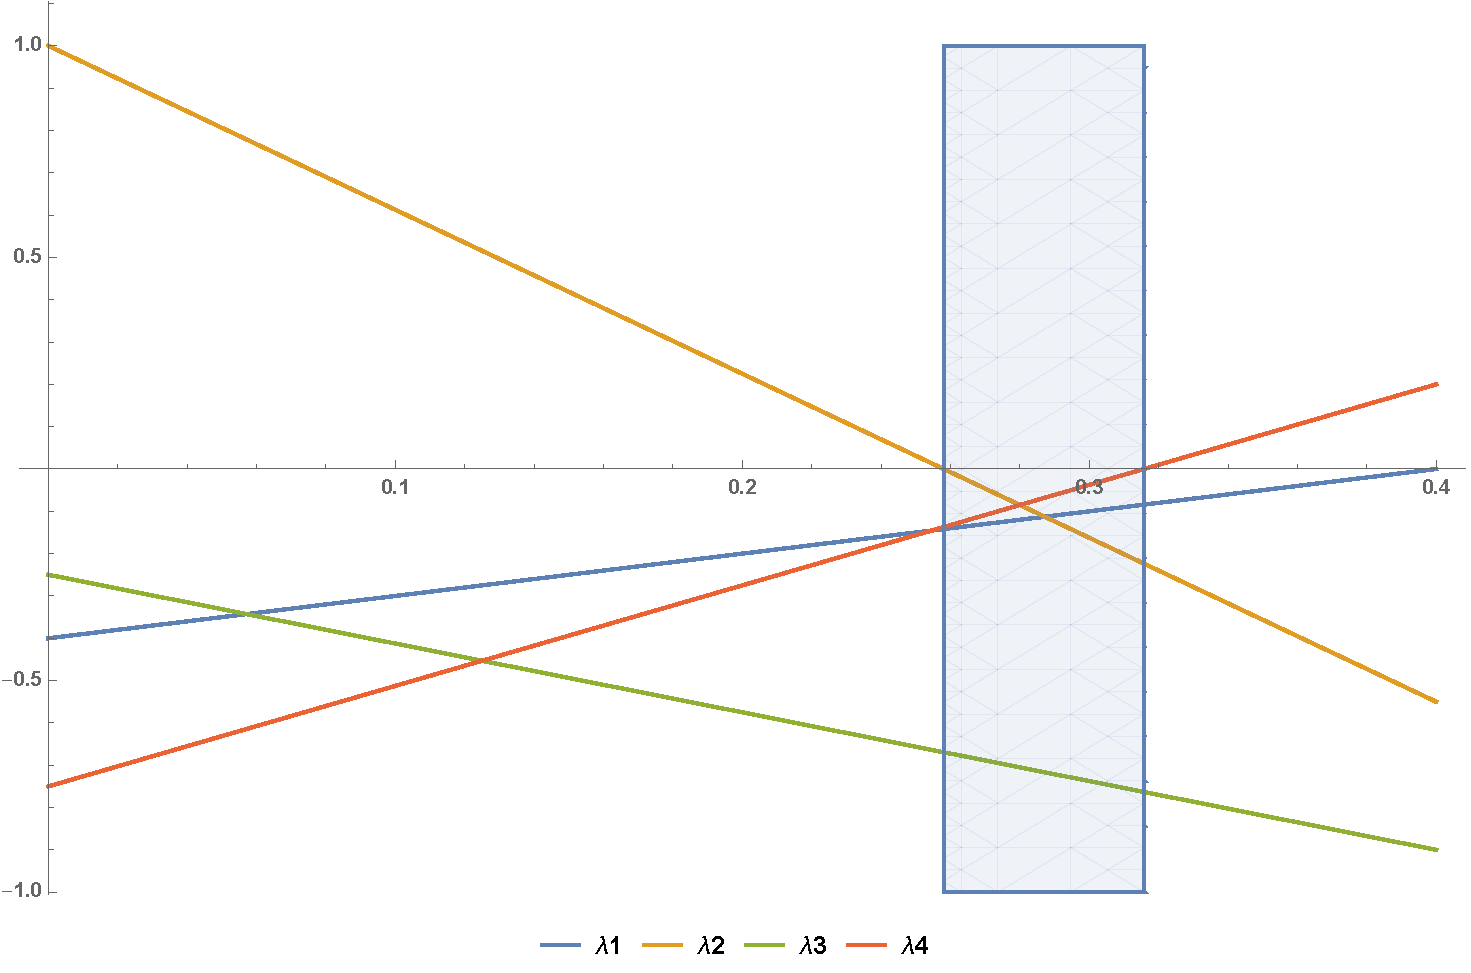
\includegraphics[width=0.9\textwidth]{EigenvalueStabilityRegion.pdf}
    \caption{The region, defined by the constraints given by McDuffie, where the cure state equilibrium will be asymptotically stable. The eigenvalues of the Jacobian (evaluated at \((0,0,\bar{z},\bar{w}\), the cure state) are plotted as functions of \(\sigma\) with all other parameters used as the constants given by McDuffie.}
    \label{fig:stabilityregion}
\end{figure}

\begin{figure}[hp]
    \centering
    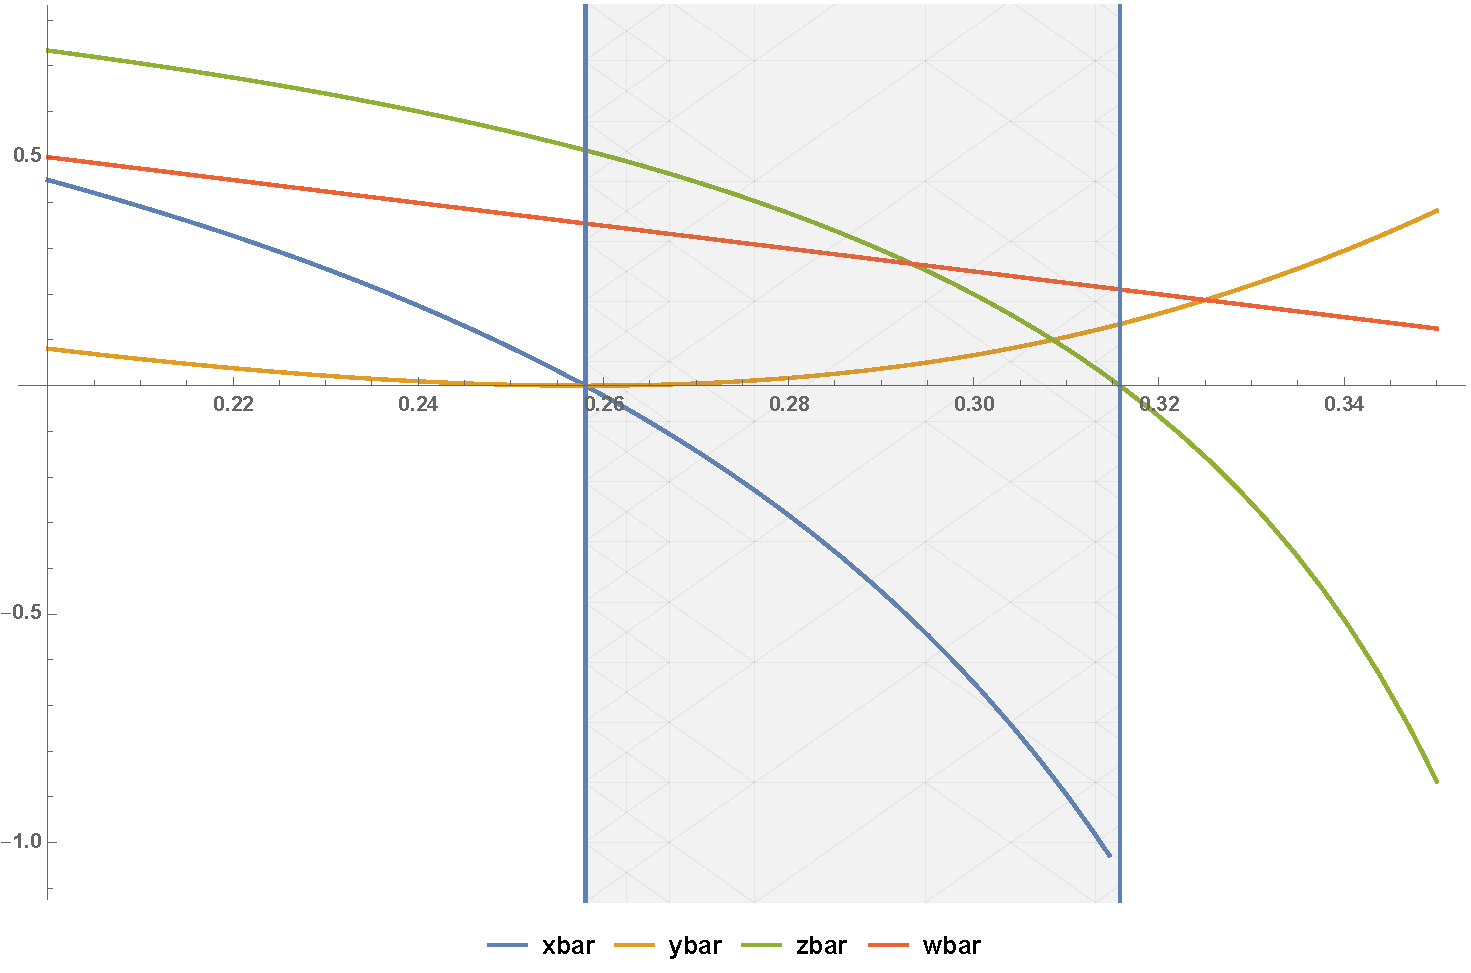
\includegraphics[width=0.8\textwidth]{ZoomedInValues.pdf}
    \caption{A close-up of the equilibrium point population values as a function of \(\sigma\). The optimal value of \(\bar{z}\) is clearly at the lower endpoint of the curve.}
    \label{fig:closeup}
\end{figure}

\begin{figure}[hp]
    \centering
    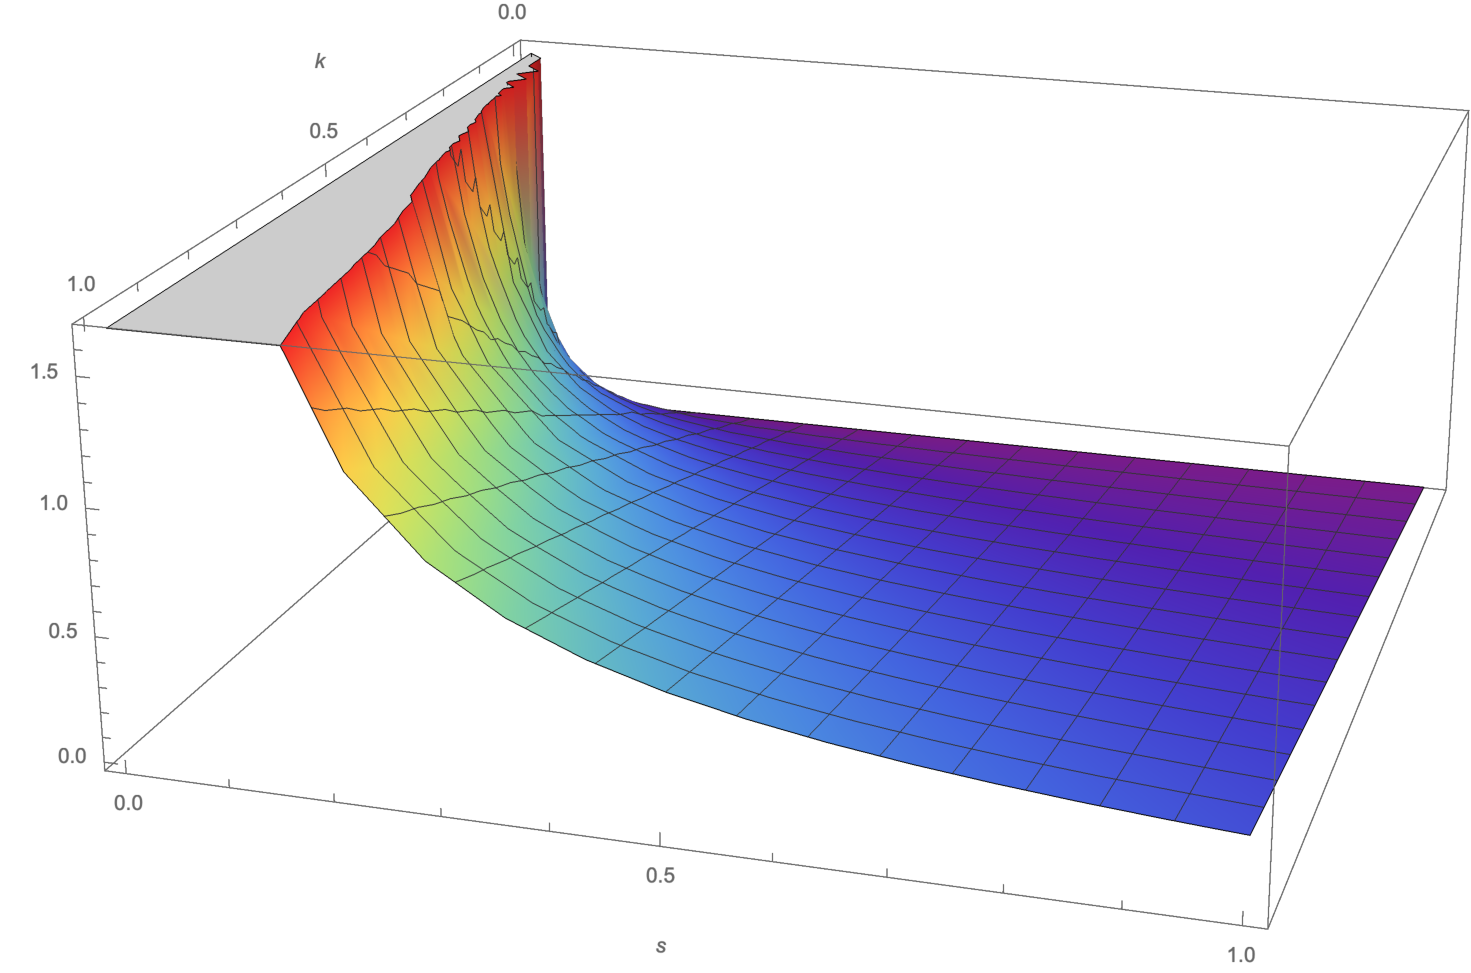
\includegraphics[width=0.8\textwidth]{DosageSurface.pdf}
    \caption{A visualization of \(D = 0.26(s/k)\) as a three-dimensional surface. Note that the surface does not plateau, but rather the surface was truncated as it spikes towards infinity as \(s\) increases and \(k\) decreases. (Interestingly, a level set of \(\sigma\), which is a 4D surface.)}
    \label{fig:dosagesurface}
\end{figure}

\end{document}
